% \NeedsTeXFormat{LaTeX2e}
\documentclass[12pt,letterpaper]{article}
\usepackage[spanish]{babel}
\usepackage[ansinew]{inputenc}
\usepackage[right=2cm,left=2cm,top=3cm,bottom=3cm,headsep=1cm,footskip=0.5cm]{geometry}
\usepackage[dvips]{graphicx}
\usepackage[nobib]{CoverPage}
\usepackage{invoice}
\usepackage{pifont}
\usepackage{xcolor}

\usepackage[T1]{fontenc} % recommended for languages with accents
% \usepackage[utf8]{inputenc}
\usepackage[latin1]{inputenc}

\usepackage[hidelinks]{hyperref}
\hypersetup{colorlinks=false}

\usepackage{fontspec}
\usepackage[misc]{ifsym}


% Awesome fonts
\usepackage{fontawesome}
% \newfontfamily{\FA}{FontAwesome Regular}
% \def\twitter{{\FA \faTwitter}}
% \usepackage[hidelinks,linkbordercolor=false]{hyperref}
% \hypersetup{
% 	colorlinks{false}
% 	urlcolor{magenta}
% 	filecolor{cyan}
% 	linkcolor{blue}
% 	linkbordercolor{false}
% 	colorlinks{false}
% }



\usepackage{pstricks}
\usepackage{pst-all}

\newpsobject{malla}{psgrid}{subgriddiv=1,griddots=10,gridlabels=6pt}

% for quotes
% \usepackage{csquotes}

% \usepackage{pstcol} % para color
% \usepackage{pst-node} % para diagramas
% \usepackage{pst-plot} % para representacion de datos
% funciones, etc


\usepackage{tocloft}
%%gmedina solution
\renewcommand{\listfigurename}{Imagenes}
\renewcommand{\listtablename}{Tablas}
\renewcommand{\contentsname}{Contenidos}

\renewcommand{\figurename}{Imagen}
\renewcommand{\tablename}{Datos}



\newcommand{\listequationsname}{Equaciones}
\newlistof{myequations}{equ}{\listequationsname}
\newcommand{\myequations}[1]{%
\addcontentsline{equ}{myequations}{\protect\numberline{\theequation}#1}\par}
\setlength{\cftmyequationsnumwidth}{2.5em}% Width of equation number in List of Equations


 \usepackage{marvosym} % telephoneicons



\usepackage{mathtools}

\usepackage{verbatim}
\usepackage{listings}
% \usepackage{color}
% \lstset{language=PHP}
% \lstset{basicstyle=\ttfamily,
%  showstringspaces=false,
%  commentstyle=\color{red},
%  keywordstyle=\color{blue}
% }
% \usepackage{listings}
% \usepackage{color}





\usepackage{fancyheadings}
% This defines some new pagestyles which you can invoke with:
% \pagestyle{fancy}
% or
\pagestyle{fancyplain}
\newcommand{\tstamp}{\today}
\renewcommand{\chaptermark}[1]{\markboth{#1}{}}
\renewcommand{\sectionmark}[1]{\markright{#1}}
\lhead[\fancyplain{}{\thepage}]         {\fancyplain{}{\rightmark}}
\chead[\fancyplain{}{}]                 {\fancyplain{}{}}
\rhead[\fancyplain{}{\rightmark}]       {\fancyplain{}{\thepage}}
\lfoot[\fancyplain{}{}]                 {\fancyplain{\tstamp}{\tstamp}}
\cfoot[\fancyplain{\thepage}{}]         {\fancyplain{\thepage}{}}
\rfoot[\fancyplain{\tstamp} {\tstamp}]  {\fancyplain{}{}}





\definecolor{mygreen}{rgb}{0,0.6,0}
\definecolor{mygray}{rgb}{0.5,0.5,0.5}
\definecolor{mymauve}{rgb}{0.58,0,0.82}
\definecolor{kblue}{HTML}{29576B}
\definecolor{kgreen}{HTML}{1A3931}
\definecolor{oblue}{HTML}{09D4FF}
\definecolor{kgray}{HTML}{3A3A3A}
\definecolor{alert}{HTML}{C21B4D}
\definecolor{blackgreen}{HTML}{687170}
\definecolor{asome}{HTML}{22a3db}

%687170
% \lstset{ %
%   backgroundcolor=\color{white},   % choose the background color; you must add \usepackage{color} or \usepackage{xcolor}
%   basicstyle=\footnotesize,        % the size of the fonts that are used for the code
%   breakatwhitespace=false,         % sets if automatic breaks should only happen at whitespace
%   breaklines=true,                 % sets automatic line breaking
%   captionpos=b,                    % sets the caption-position to bottom
%   commentstyle=\color{mygreen},    % comment style
%   deletekeywords={...},            % if you want to delete keywords from the given language
%   escapeinside={\%*}{*)},          % if you want to add LaTeX within your code
%   extendedchars=true,              % lets you use non-ASCII characters; for 8-bits encodings only, does not work with UTF-8
%   frame=single,	                   % adds a frame around the code
%   keepspaces=true,                 % keeps spaces in text, useful for keeping indentation of code (possibly needs columns=flexible)
%   keywordstyle=\color{blue},       % keyword style
%   language=Octave,                 % the language of the code
%   otherkeywords={*,...},            % if you want to add more keywords to the set
%   numbers=left,                    % where to put the line-numbers; possible values are (none, left, right)
%   numbersep=5pt,                   % how far the line-numbers are from the code
%   numberstyle=\tiny\color{mygray}, % the style that is used for the line-numbers
%   rulecolor=\color{black},         % if not set, the frame-color may be changed on line-breaks within not-black text (e.g. comments (green here))
%   showspaces=false,                % show spaces everywhere adding particular underscores; it overrides 'showstringspaces'
%   showstringspaces=false,          % underline spaces within strings only
%   showtabs=false,                  % show tabs within strings adding particular underscores
%   stepnumber=2,                    % the step between two line-numbers. If it's 1, each line will be numbered
%   stringstyle=\color{mymauve},     % string literal style
%   tabsize=2,	                   % sets default tabsize to 2 spaces
%   title=\lstname                   % show the filename of files included with \lstinputlisting; also try caption instead of title
% }


\lstdefinestyle{customc}{
  belowcaptionskip=1\baselineskip,
  breaklines=true,
  frame=L,
  xleftmargin=\parindent,
  language=PHP,
  showstringspaces=false,
  basicstyle=\footnotesize\ttfamily,
  keywordstyle=\bfseries\color{blue!40!black},
  commentstyle=\itshape\color{mymauve!40!black},
  identifierstyle=\color{blue},
  stringstyle=\color{mygreen},
  numberstyle=\tiny\color{mygray},
}

%-----------------------------------------------------------------------
% after parsing the BibTeX data and reading the "CoverPage.cfg"
% config file, you can manually setup the cover main in your main
% document:
% \emph{elephantom.soporte@gmail.com}
\CoverPageSetup{title=Administraci\'on de Transporte,author=Departamento de Desarrollo y Consultor\'ia ,institute={\copyright{elephantom}},insource={\href{mailto:elephantom.soporte@gmail.com}{\faEnvelopeO\ \emph{elephantom.soporte@gmail.com}} \\ \href{http://elephantom.xyz}{\faExternalLink\ \emph{www.elephantom.xyz}} },copyright={\copyright{elephantom} } }
% \CoverPageSetup{institute=C,insource=D,copyright=E}
% this line would create an automatic IEEE copyright notice
\CoverPageSetup{year=2017,publisher=Elephantom.Inc}
% \CoverPageSetup{year=2017,publisher=IEEE}
% and settings like this set the source; booktitle would also work
% \CoverPageSetup{journal=\textit{El sistema se divide en cuatro m\'odulos, un sistema de logueo y un historial de procesos}}
% Of course, all necessary keys can be combined in a single
% \CoverPageSetup command.

% \CoverPageSetup{institute = {Institute of Applied Computer Science}}
% \renewcommand{\CoverPageHeader}{%
% 
\includegraphics[width=\textwidth]{img/elephantom_transparent.png}
% }

\renewcommand{\CoverPageHeader}{%
%  {\includegraphics[width=.20\textwidth]{geonext.png}}%
  {
  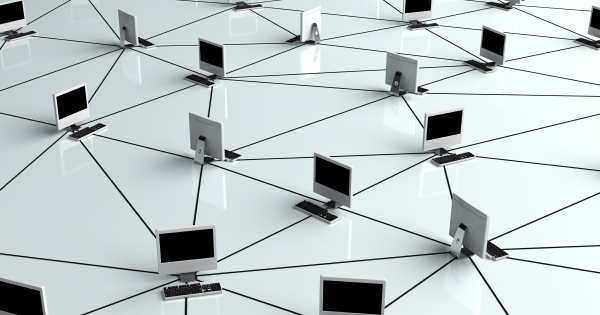
\includegraphics[width=160mm]{img/nas_net.jpg}}%
  }
  % \LARGE\bfseries%
  % \hrulefill{} {\color{green}HEADER LOGO} \hrulefill}
% \renewcommand{\CoverPageFooterLogo}{%
%   \Huge\sffamily%
%   {\color{blue}L-O-G-O}}
% \renewcommand{\CoverPageBody}{\includegraphics[width=.35\textwidth]{rwthlogo}}
% \renewcommand{\CoverPageFooter}{\includegraphics[width=.35\textwidth]{rwthlogo}}

\renewcommand{\CoverPageFooterLogo}{
\includegraphics[width=.15\textwidth]{img/elephantom_transparent.png}}
%-----------------------------------------------------------------------
\begin{document}
  {
	\sffamily % Start the Document
	% for smallcaps shape use the command \scshape
	\title{Servicios en la Nube}
	\author{\copyright elephantom}
	\maketitle
	\tableofcontents
	% \listoffigures
	% \listofmyequations
	%   \makeglossaries
	\newpage
  }

  \begin{section}{\color{kblue}\sffamily{Propuesta de trabajo}}
  	\begin{subsection}{\color{blackgreen}\sffamily{Modelo 1}}
  	\sffamily
  	{

    \subsubsection{Servidor en la nube}
    El esquema en la nube es un modelo practico que trae ahorro para el cliente ya que evita inversiones recurrentes en administrar el software, los servidores, equipos, redes e infraestructura para poder operar de manera eficiente la solución.
    La solución estará disponible para acceder a ella desde cualquier computadora con Internet.

    \subsubsection{Servicios}
      \begin{figure}[htb]
        \centering
        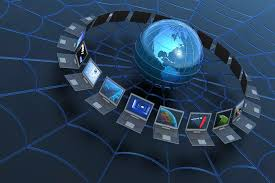
\includegraphics[angle=0,width=140mm,height=90mm]{img/images_net.jpeg}
        \caption{Servicios en la nube}
        \label{sel064}
      \end{figure}


      \begin{itemize}
        \item[\ding{182}]
        {
          Conexi\'on directa a soluci\'on v\'ia Internet
        }
        \item[\ding{183}]
        {
          Software.- Sistema dedicado y hecho para transporte, se maneja la versi\'on est\'andar y comercial.
        }
        \item[\ding{184}]
        {
          Infraestructura.-Servidor  en Alemania, administrado,cuenta con respaldos diarios de la base de datos y ejecuci\'on peri\'odica de planes de mantenimiento \textbf{desempeño de la red} 100Mb de velocidad.
        }
      \item[\ding{185}]
      {
        Costos y Plazo.- Costo mensual de \$10,000.00   (Diez mil pesos 00/100 M.N.) + IVA (factura expedida por \textbf{Servicios profesionales – Asesor\'ia o consultor\'ia}
        En caso de querer terminar la relaci\'on se entrega una base de datos con toda la informaci\'on generada hasta el momento.
      }
      \item[\ding{186}]
      {
        Capacitaci\'on.- La capacitaci\'on y el uso del sistema es de manera remota en propuesta los d\'ias s\'abados en horario de 10 a.m. a 12 p.m. (o a acordar) se entregan manuales de todos los m\'odulos en su versi\'on \texbf{pdf} y se brinda asesor\'ia en caso de dudas en los t\'erminos o procesos.
      }
      \item[\ding{187}]
      {
        Reportes.-Se entregan 2 reportes \textbf{a modo} a solicitud del cliente, esto es al tener tres meses de trabajo para poder tener informaci\'on y realizar validaciones (requerimiento documentado).
      }
      \item[\ding{188}]
      {
        Formatos.- Los formatos (por ejemplo Cartas de porte,Vales de diesel, Anticipos) son las versiones est\'andar de la soluci\'on. (se puede generar una muestra de impresi\'on)
      }
      \item[\ding{189}]
      {
        Soporte.-Soporte por medio de sistema de tickets con el fin de ejemplificar a detalle el problema en cuesti\'on. Algunas modificaciones ser\'an v\'ia Base de datos, con previa autorizaci\'on del responsable y contacto. Horario de 9:00 a.m. a 5:30 p.m. de Lunes a Viernes
      }
      \item[\ding{190}]
      {
        Desarrollos .- El desarrollo de reportes o interface con otros sistemas sera con previa solicitud, documentaci\'on (alcances) y an\'alisis con el desarrollador , esto es considerado independiente a la propuesta de trabajo en su esquema y costos.
      }
      \item[\ding{191}]
      {
        Otros.- En caso de existir un tema a tratar quedamos abiertos.
      }
      \end{itemize}
    }
  \end{section}

\newpage
\begin{section}{\color{kblue}\sffamily{M\'odulos}}

	\begin{subsection}{\color{blackgreen}\sffamily{.NET}}
	\sffamily
	{
    \subsubsection{OperacionesV6}
      Controla todo el proceso operativo desde la solicitud del viaje  hasta la entrega del pedido con el cliente
    \subsubsection{LlantasNet}
      Administra la rotaci\'on y uso de tus llantas , su rendimiento y costos de renovaci\'on
    \begin{subsection}{\color{blackgreen}\sffamily{PBD}}

    \subsubsection{Mantenimiento}
      Controla los gastos y refacciones de cada unidad , las actividades de los mec\'anico , muestra informaci\'on de los rendimientos de combustible.
      Y dise\~na tus propios ciclos de mantenimiento preventivo. Gestiona las ordenes de taller externo
    \subsubsection{Tr\'afico}
      Genera las liquidaciones de los viajes de cada operador.
    \subsubsection{Facturaci\'on y Cobranza (clientes)}
      Realiza las facturas de fletes u otros ingresos , controla la cartera y proyecci\'on de clientes.
    \subsubsection{Accidentes (p\'olizas)}
      Lleva un control de las p\'olizas de tus unidades , registra los accidentes.
    \subsubsection{Almac\'en}
      Gestiona la rotaci\'on de tus refacciones , entradas ,salidas y cardex
  \footnotesize{\scshape{
      Los M\'odulos PBD requieren ser ejecutados en la computadora cliente por lo que se requiere una modificaci\'on extra para crear un \textbf{túnel} que funcionara como VPN con conexi\'on directa al servidor.
    }
  }

	}
	\end{section}


  \begin{section}{\color{kblue}\sffamily{Requisitos M\'inimos de Hardware}}

  	\sffamily
  	{
    \begin{subsection}{\color{blackgreen}\sffamily{Workstations :}}

      \begin{itemize}
        \item[\ding{182}]
        {
          Procesador : 1.5 ghz
        }
        \item[\ding{183}]
        {
          N\'ucleos del procesador : 2
        }
        \item[\ding{184}]
        {
          Memoria : 2GB
        }
        \item[\ding{185}]
        {
          Espacio en Disco : 3GB
        }
        \item[\ding{186}]
        {
          Tarjeta de Red : 100 mb/s
        }
        \item[\ding{187}]
        {
          Sistema Operativo : \copyright{Windows 7} \footnote{La versi\'on de Windows puede ser anterior, depende del m\'odulo a trabajar}
        }
        \item[\ding{188}]
        {
          Acceso a internet
        }
      \end{itemize}
    }
  \end{section}




\newpage
  \begin{section}{\color{kblue}\sffamily{Nuestra experiencia}}
  \sffamily
  {

  \begin{itemize}
    \item[\ding{182}]
    {
      Contamos con 9 a\~nos de experiencia en Transporte
    }
    \item[\ding{183}]
    {
      Implementaci\'on y consultor\'ia del sistema en diferentes tipos operaci\'on.
    }
    \item[\ding{184}]
    {
      Adem\'as de 15 a\~nos de experiencia en desarrollo de software (Php,Python,.NET,etc) \\ somos capaces de desarrollar en diferentes tipos de lenguaje y plataformas.
    }
    \item[\ding{185}]
    {
      Tambien Manejamos y administramos todo tipo de Bases de Datos.
    }
    \item[\ding{186}]
    {
      Manejo de ERPs\\Microsoft Reporter for Microsoft Dinamycs ERP (SL)\\Oddo (OpenERP)
    }

    % \subsection{Contamos con 9 a\~nos de experiencia en Transporte}
    %
    % \subsection{Implementaci\'on y consultor\'ia del sistema en diferentes tipos operaci\'on.}
    %
    % \subsection{Adem\'as de 15 a\~nos de experiencia en desarrollo de software (Php,Python,.NET,etc) \\ somos capaces de desarrollar en diferentes tipos de lenguaje y plataformas.}
    %
    % \subsection{Tambien Manejamos y administramos todo tipo de Bases de Datos.}
    %
    % \subsection{Manejo de ERPs\\Microsoft Reporter for Microsoft Dinamycs ERP (SL)\\Oddo (OpenERP)}
  }
  \end{section}

  \newpage
    \begin{section}{\color{kblue}\sffamily{Glosario}}
    \sffamily
    {
      \subsection{Interface} Es el canal por que cual se Env\'ia y recive informaci\'on que permite comunicarse a los sistemas (ERP) entre si, con el fin de optimizar y agilizar los recursos de los sistemas.\\
      \subsection{Tunnel} Es una tecnolog\'ia de red de computadoras que permite una extensi\'on segura de la red de \'area local (LAN) sobre una red p\'ublica o no controlada como Internet.
      Permite que la computadora en la red env\'ie y reciba datos sobre redes compartidas o p\'ublicas como si fuera una red privada con toda la funcionalidad, seguridad y
      pol\'iticas de gesti\'on de una red privada.
      Esto se realiza estableciendo una conexi\'on virtual punto a punto mediante el uso de conexiones dedicadas, cifrado o la combinaci\'on de ambos métodos.
    }
    \end{section}

    \newpage
      \begin{section}{\color{kblue}\sffamily{Contacto}}
      \sffamily
      {
        Ing. Javier Garcia Vargas \\
        \color{asome}\faMobile\ (01) 272-116-91-95 \\
        \href{mailto:elephantom.soporte@gmail.com}{\color{asome}\faEnvelope\ \emph{elephantom.soporte@gmail.com}} \\
        \href{http://elephantom.xyz}{\color{asome}\faCloud\ \emph{www.elephantom.xyz}} \\
      }
      \end{section}

%
% \newpage
%   \begin{section}{\color{kblue}\sffamily{Add Document}}
%   \sffamily
%   {
%
%   }
%   \end{section}



% FOR FOOTNOTES
  % \footnotesize{\scshape{}}

% FOR TABLES
% \begin{table}
% \end{table}

% EQUATIONS
% \begin{equation}
% 	costoLlamada = { totalDeMinutos x tarifa[codigoDePais] }
% 	\label{eq:costo de la llamada}
% \end{equation}
%
% \myequations{costo_call}

\end{document}
